% Created 2021-09-12 Sun 22:49
% Intended LaTeX compiler: xelatex
\documentclass[letterpaper]{article}
\usepackage{graphicx}
\usepackage{grffile}
\usepackage{longtable}
\usepackage{wrapfig}
\usepackage{rotating}
\usepackage[normalem]{ulem}
\usepackage{amsmath}
\usepackage{textcomp}
\usepackage{amssymb}
\usepackage{capt-of}
\usepackage{hyperref}
\usepackage[margin=1in]{geometry}
\usepackage{fontspec}
\usepackage{indentfirst}
\setmainfont[ItalicFont = LiberationSans-Italic, BoldFont = LiberationSans-Bold, BoldItalicFont = LiberationSans-BoldItalic]{LiberationSans}
\newfontfamily\NHLight[ItalicFont = LiberationSansNarrow-Italic, BoldFont       = LiberationSansNarrow-Bold, BoldItalicFont = LiberationSansNarrow-BoldItalic]{LiberationSansNarrow}
\newcommand\textrmlf[1]{{\NHLight#1}}
\newcommand\textitlf[1]{{\NHLight\itshape#1}}
\let\textbflf\textrm
\newcommand\textulf[1]{{\NHLight\bfseries#1}}
\newcommand\textuitlf[1]{{\NHLight\bfseries\itshape#1}}
\usepackage{fancyhdr}
\pagestyle{fancy}
\usepackage{titlesec}
\usepackage{titling}
\makeatletter
\lhead{\textbf{\@title}}
\makeatother
\rhead{\textrmlf{Compiled} \today}
\lfoot{\theauthor\ \textbullet \ \textbf{2021-2022}}
\cfoot{}
\rfoot{\textrmlf{Page} \thepage}
\titleformat{\section} {\Large} {\textrmlf{\thesection} {|}} {0.3em} {\textbf}
\titleformat{\subsection} {\large} {\textrmlf{\thesubsection} {|}} {0.2em} {\textbf}
\titleformat{\subsubsection} {\large} {\textrmlf{\thesubsubsection} {|}} {0.1em} {\textbf}
\setlength{\parskip}{0.45em}
\renewcommand\maketitle{}
\author{Houjun Liu}
\date{\today}
\title{Bacterial Infections}
\hypersetup{
 pdfauthor={Houjun Liu},
 pdftitle={Bacterial Infections},
 pdfkeywords={},
 pdfsubject={},
 pdfcreator={Emacs 28.0.50 (Org mode 9.4.4)}, 
 pdflang={English}}
\begin{document}

\maketitle


\section{Bacterial Infections}
\label{sec:org6fbd110}
Induction of diseases via the entry of bacteria.

\begin{itemize}
\item \textbf{Bacterial-induced toxicity} => produces toxins + has hard capsule
cell
\item \textbf{Host-mediated factors} => may develop host resistance, could compete
for resources, and could be grown introcellularly
\end{itemize}

\subsection{Biofilm formation}
\label{sec:orgc5b8d8c}
\begin{itemize}
\item Communities of bacteria could work together by adhering and exchanging
information
\item Bacterial could perform quorum sensing => exchange of information with
each other + recognize various members of their group
\end{itemize}

\subsection{Fighting bacterial infections}
\label{sec:orgbee9dfd}
\textbf{Antibiotics} => drugs with selective toxicity for specific bacterial
types

Act by\ldots{}

\begin{itemize}
\item Disrupting membrane + cell wall integrity
\item Selectively target + impair bacterial ribosomes
\item Block bacterial DNA replication/transcription
\item Inhibit bacterial metabolism
\end{itemize}

\href{https://drive.google.com/file/d/1WRnbgkhnmRrdP4ZqlqT3HHBD1\_eW9qib/view}{This
video}

\begin{figure}[htbp]
\centering
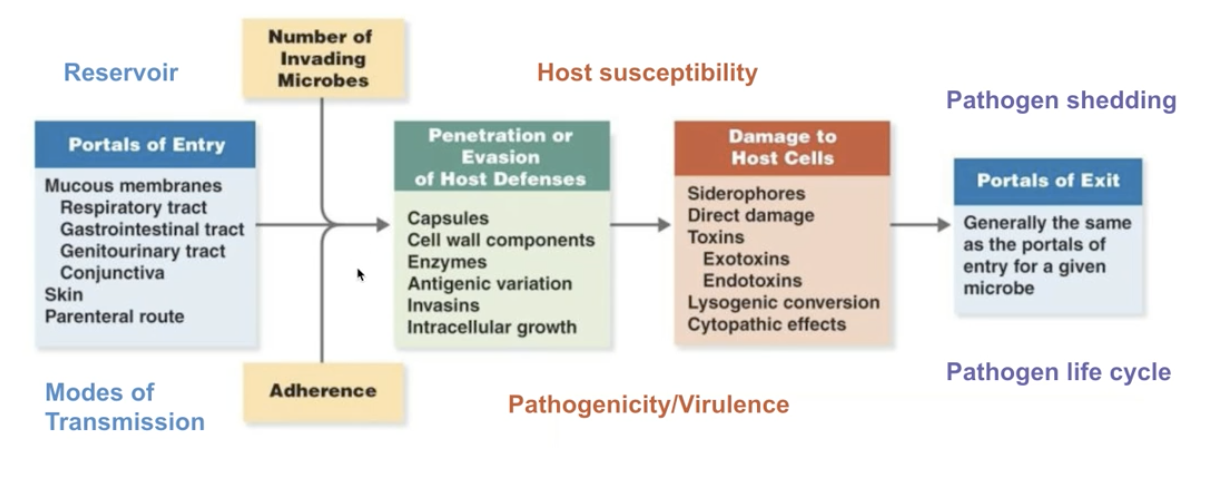
\includegraphics[width=.9\linewidth]{Screen Shot 2020-10-12 at 3.08.53 PM.png}
\caption{Screen Shot 2020-10-12 at 3.08.53 PM.png}
\end{figure}
\end{document}
